\chapter{Microservices}

Der Begriff Microservices stifte derzeit noch große Verwirrung. Nicht nur weil er relativ neu ist, sondern auch weil er sehr breit gefächert ist und eine klare Abgrenzung kaum möglich ist. Im nachfolgenden Kapitel wird der Begriff Microservice ausführlich definiert, beschrieben und zu anderen Konzepten abgegrenzt.

\section{Was ist ein Microservice}

Hinter Microservices verbirgt sich keine Technologie die aktiv entwickelt wurde. Vielmehr ist es ein Sammelbegriff der nachträglich für über die Jahre entstandener Praktiken, Methoden und Technologien, im Umfeld von komplexen Softwaresystemen, eingeführt wurde. Am häufigsten ist mit Microservices die sogenannte Microservice Architektur gemeint. Charakteristisch für dieses Softwarearchitekturmuster ist die Zerlegung eines Softwaresystems in kleine, autonome Dienste, die mit einem leichtgewichtigem Kommunikationsprotokoll miteinander interagieren, zu einem zu einem verteilten System. Die Fähigkeiten eines einzelnen Dienstes ist genau auf die Geschäftsanforderungen eines bestimmten Unternehmens oder Einsatzgebietes zugeschnitten \cite{FowlerMS}. Die Verwendung dieses Muster bringt aber neben technischen Einflüssen, meistens auch organisatorische Einflüsse mit sich. Beispielsweise auf die Teamstruktur, Verantwortung, Continuous Integration, Testing, um nur einige davon zu nennen. Daher können mit den Begriff Microservices viele verschiedene Aspekte gemeint sein.

Um zu verstehen warum sich Microservices derart großer Beliebtheit erfreuen, ist es notwendig zu verstehen, wie die Architektur derartiger Systeme vor diesem Paradigmenwechsel ausgesehen hat. Dazu beschreibt der nächste Abschnitt den sogenannten monolithischen Ansatz und welche Probleme damit verbunden sind, die durch Microservices gelöst werden.

\subsection{Monolithische Ansatz}

Mittlerweile haftet der monolithischen Softwarearchitektur, zu unrecht, ein negativer Ruf an. Obwohl dieser Ansatz seit Jahrzehnten  in vielen Bereichen der Softwareindustrie sehr gut funktioniert. Im Java und .NET Umfeld war \bzw ist dieser Ansatz noch immer gängige Praxis. Dennoch wird er vielerorts von der Microservice Architektur abgelöst. Doch was macht eine Anwendung überhaupt zu einem Monolithen?

Unter einem Monolithen versteht man in der Softwareentwicklung eine Anwendung, in der verschiedene Geschäftsbereiche oder Funktionalitäten als eine einzige Anwendung zusammengeschlossen sind \cite{FowlerMS}. Intern kann die Applikation beispielsweise als Mehrschicht-Architektur organisiert sein. Üblich sind hier folgende drei Schichten \cite{FowlerPEA}:

\begin{itemize}
	\item \textbf{Präsentationsschicht:} Hier ist derjenige Quelltext angesiedelt, der sich mit der Darstellung der Benutzerschnittstelle, \zB als Web- oder Desktopanwendung auseinandersetzt.
	\item \textbf{Geschäftslogikschicht:} Diese Schicht stellt den Kern der Anwendung dar. Sie enthält alle Geschäftsrelevanten Funktionen.
	\item \textbf{Datenzugriffsschicht}: In dieser Schicht befinden sich die Funktionalität die zum Zugriff auf externen Datenquellen, wie \zB relationale Datenbanken, notwenidg ist.
\end{itemize}


In Abbildung \ref{fig:layered-architecture} ist der Aufbau eines Monolithen mit Drei-Schicht-Architektur skizziert. Der Zugriff darf jeweils nur auf die direkt darunterliegende Schicht erfolgen. Innerhalb jeder Schicht ist eine Modularisierung in verschiedene Bereiche, die auf die Geschäftsfunktionen abgestimmt sind, sinnvoll.

\begin{figure}[!htb]
\centering
\minipage{0.5\textwidth}
  \centering
	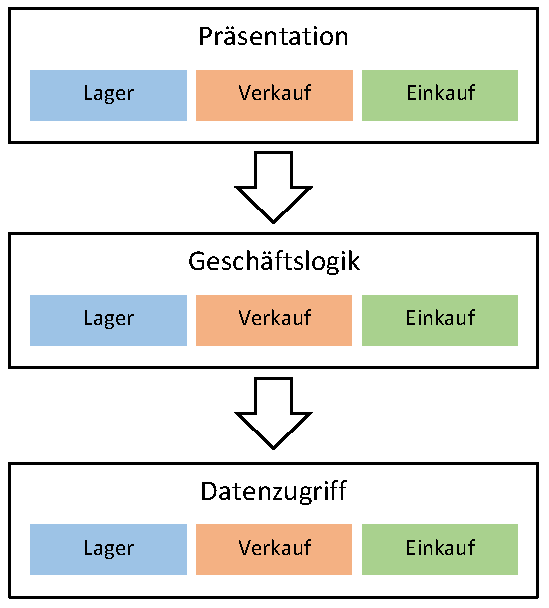
\includegraphics[width=0.8\linewidth]{layered-architecture}
	\caption{Drei-Schicht-Architektur}
	\label{fig:layered-architecture}
\endminipage
\minipage{0.5\textwidth}
  \centering
	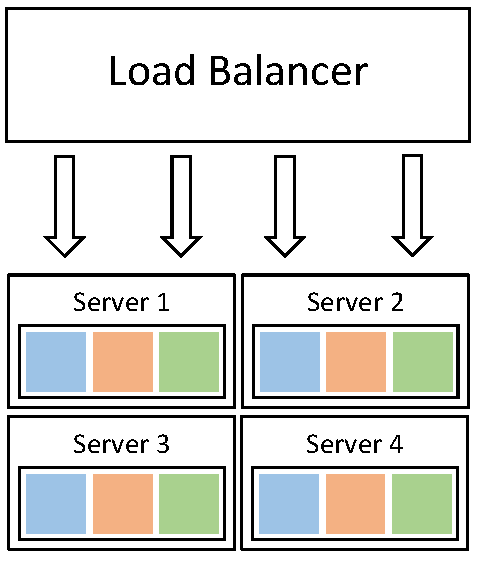
\includegraphics[width=0.76\linewidth]{monolith-scale}
	\caption{Skalieren eines Monolithen}
	\label{fig:monolith-scale}
\endminipage
\end{figure}

\subsubsection{Nachteile und Schwierigkeiten}

Mit steigender Komplexität kommen nach und nach Probleme zum Vorschein, der diesen Ansatz aufwändig oder sogar unpraktikabel machen. Eines der Hauptprobleme ist bei Internetweiten Anwendungen die Skalierbarkeit. Die einzige Möglichkeit einen Monolithen zu skalieren ist auf mehreren Servern jeweils eine Instanz des Monolithen zu installieren und über einen Load-Blancer zu verbinden. Abbildung \ref{fig:monolith-scale} zeigt wie ein solcher Aufbau aussehen kann. In vielen Einsatzgebieten ist dieser Ansatz aber nicht feingranular genug. Oft ist es sinnvoller nur bestimmte Teile es Gesamtsystems zu skalieren.

Ein Monolith stößt aber nicht nur aus technischer Sichtweise auf Skalierbarkeitsprobleme, sondern auch aus organisatorischer Sicht. Alle Entwickler arbeiten zwangsläufig an der gleichen Codebasis, die dadurch enorme Größe annehmen kann. Kein einzelner Entwickler ist mehr in der Lage die ganze Codebasis zu überblicken und zu beurteilten welche Auswirkung eine Änderung haben kann. Das führt über kurz oder lang zur Verlangsamung der Entwicklungsgeschwindigkeit oder sogar zu völligem Stillstand.

Vor allem in Technologiebranche ändern sich Anforderungen sehr rasch. Agile Softwareprozesse unterstützen dabei, die geänderten Anforderung so schnell es geht in die Software einfliessen zu lassen. Für den Kunden \bzw Endbenutzer zählt nur die schnellstmögliche Umsetzung seiner neuen Anforderungen. In einem Monolithen sind mehrere Geschäftsbereiche zusammengefasst. Der Monolith muss immer als ganzes getestet und ausgerollt werden. Dadurch verlangsamt sich der gesamte Releasezyklus auf den langsamsten Teilbereich, obwohl vielleicht der Teilbereich in dem eine Änderung notwendig war, schon längst fertiggestellt ist.

Hinter einem Monolith steht immer eine bestimmte Technologie oder eine Sammlung von mehreren Technologien, wie \zB Java EE oder ASP.NET. Somit müssen alle Teilbereiche der Anwendung auf die selben Technologien zurückgreifen. Für manche Teilbereiche könnte aber möglicherweise die Verwendung von alternativen Technologien und Speichersystemen große Vorteile bringen.

In diesem Abschnitt wurden einige der Hauptkritikpunkte am monolithischen Architekturmuster angeführt. Es mag den Anschein vermittelt haben, dass dieser Ansatz nicht mehr verwendet werden soll. Im Gegenteil. Viele Experten sind der Meinung, dass gerade am Anfang eines Projekts der monolithische Ansatz zu bevorzugen ist \cite{FowlerMolithFist}. Erst nachdem das Verständnis für die Domäne vorhanden ist und Anforderungen klarer sind, ist der Übergang zu einer Microservice Architektur leichter und sinnvoll. 

\section{Charakteristiken eines Microservice}

Dieser Abschnitt beschreibt einige charakteristische Merkmale eines Microservice. Wie bereits erwähnt gibt es keine eindeutige Definition eines Microservice. Daher ist es sinnvoller, allgemeine anerkannte Charakteristiken der Microservice Architektur zu betrachten, die durch die meisten Definitionen beschrieben werden. 
\citeauthor{FowlerMS} identifizierte in \cite{FowlerMS} neun Charakteristiken eines Microservice. Obwohl diese Liste bereits sehr exhaustiv ist, sind immer wieder sinnvolle Ergänzungen, wie in \cite{HorsdalMS} zu finden. Die nachfolgenden Abschnitten gehen etwas detaillierter auf einige essentielle Merkmale ein.

\subsection{Organisation um Geschäftskompetenzen}

Normalerweise sind Softwareentwicklungsteams anhand ihrer technologischen Spezialisierung in Teams eingeteilt:

\begin{itemize}
	\item Front-End Entwickler
	\item Backend-End Entwickler
	\item Datenbank-Administatoren
	\item IT-Administator
\end{itemize}

Durch die Microservice Kultur hat sich aber eine andere Art der Teamstrukturierung etabliert. Für jede Geschäftskompetenz ist genau ein Team, welches intern aus einer kleinen Anzahl an den eingangs genannten Technologieexperten besteht, verantwortlich. Damit soll die Identifizierung und das Verantwortungsbewusst sein jedes einzelnen Teammitglieds für das von ihm entwickelte und betriebene Produkt stärken.

Was aber dennoch eine große Herausforderung bleibt, ist die Definition des Aufgabenbereichs eines einzelnen Teams. Die Identifikation und Abgrenzung der Geschäftskompetenzen eines Unternehmens ist eine sehr komplexe Aufgabe. Als Hilfsmittel lässt sich hier das \begin{english} Single-Responsibility-Principle\end{english} heranziehen \cite{MartinAgile}: 

\begin{english}
\begin{quote}
  \textit{A class should have only one reason to change.}
\end{quote}
\end{english}

Das aus der objektorientierten Programmierung bekannte Design-Prinzip kann auch im Kontext von Microservices angewandt erden. Es erweitert diesen Grundsatz von der Klassen-Ebenen auf die Dienst-Ebene. Das heißt für jeden Dienst soll genau eine Fähigkeit realisieren. Damit ist sichergestellt, dass geänderte Geschäftsanforderungen so wenig Dienste wie notwendig beeinflussen.

\subsection{Modularisierung durch Dienste}
\label{subsec:Componentization}

Seit Jahrzehnten strebt die Softwareenwicklungsbranche danach, komplexe Softwaresysteme einfach durch die Integration verschiedener Komponenten realisieren zu können. Durch dieses Jahrelange bestreben und unterschiedlichste Ansätze ist leider auch der Begriff Komponente sehr überstrapaziert und hat dementsprechend viele unterschiedliche Bedeutungen. Beispielsweise in der objektorientierten Programmierung kann eine Klasse als Komponente betrachtet werden. Darüber hinaus gibt es noch viele weitere Bedeutungen.

Auch wenn die konkrete Umsetzung einer Komponente sehr vielfältig sein kann, haben alle Arten die selben Ziele:

\begin{itemize}
	\item \textbf{Austauschbarkeit:} Es soll möglich sein, eine Komponenten durch eine andere zu ersetzen. 
	\item \textbf{Wiederverwendbarkeit:} Komponenten sollen einmal entwickelt, in anderen Systemen wiederverwendet werden können.
	\item \textbf{Aktualisierbarkeit:} Durch die Austauschbarkeit ist es automatisch möglich, eine Komponente durch eine neuere Version zu ersetzen.
\end{itemize}

Im Kontext der monolithischen Softwarearchitektur sind am häufigsten die Begriffe Modul oder Software-Bibliothek stellvertretend für den Begriff Komponente. Eine Anwendung besteht somit aus einer Menge von Modulen die miteinander verbunden sind. Leider erfüllt dieser Ansatz die zuvor beschriebenen gewünschten Eigenschaften der Komponenten-Orientierung nicht ganz zufriedenstellend. Abhängigkeiten zwischen den einzelnen Modulen oder bestimmte Voraussetzungen an das Laufzeitsystem des Monolithen können es schnell verhindert, ein Modul zu aktualisieren. Somit sind die verwendeten Komponenten nicht völlig voneinander unabhängig, sondern haben versteckte Einschränkungen.

In einer Microservice-Architektur ist mit Komponente ein einzelner Dienst gemeint. Damit ist jede Komponente einer eigener Prozess, der über irgendein Kommunikationsprotokoll mit anderen Komponenten interagiert. Mit diesem Ansatz lassen sich die gewünschten Eigenschaften viel leichter realisieren.

\subsection{Dezentrale Datenverwaltung}

Eine monolithische Applikation legt sehr häufig alle persistenten Daten in einer einzigen, \zB relationalen, Datenbank ab. In einer Microservice Architektur ist dieser Ansatz nicht mehr empfehlenswert. Jede Datentyp sollen nur von einem Dienst verwaltet werden und nicht einfach direkt von einem anderen Dienst aus der Datenbank gelesen werden. Dadurch werden die Abhängigkeiten auf ein Minimum reduziert, denn andere Dienste können nur über die Schnittstelle des bereitstellenden Dienstes Daten abfragen und manipulieren. Dieses Anti-Pattern ist noch einmal in Abbildung \ref{fig:central-datastore} verdeutlicht.

\begin{figure}[h]
  \centering
	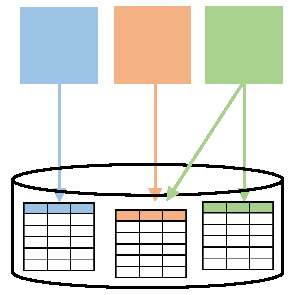
\includegraphics[width=0.3\textwidth]{central-datastore}
	\caption{Zentraler Datenspeicher}
	\label{fig:central-datastore}
\end{figure}

Wenn jeder Dienst, wie in Abbildung \ref{fig:polyglot-persistnace}, seinen eigenen Datenspeicher besitzt, kann für die Erfüllung seiner Aufgabe der optimale Speichermechanismus ausgewählt werden. Beispielsweise können Daten mit komplexen Beziehung in einer Graphendatenbank abgelegt werden. Jedoch einfache Daten in einem schnellen Key-Value-Speicher.

\begin{figure}[h]
  \centering
	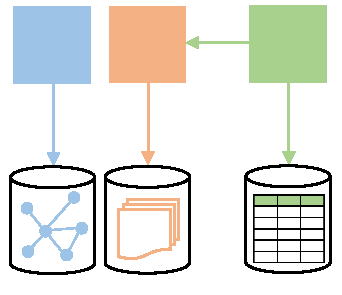
\includegraphics[width=0.3\textwidth]{polyglot-persistance}
	\caption{Polyglot Persistance}
	\label{fig:polyglot-persistnace}
\end{figure}

Auch ein Monolith könnte Gebrauch von mehreren Datenbanken machen. Dieser Ansatz ist unter dem Namen Polyglot Persistence bekannt \cite{FowlerPP}. Aus teilweise sehr vielfältigen Gründe ist er aber selten anzutreffen. Nachfolgend nur ein kleiner Auszug:

\begin{itemize}
  \item Die IT-Strategie einiger Unternehehmen sehen nur die Verwendung ganz bestimmter Datenbanken vor.
	\item Bereits getätigte Investitionen in bestehende Datenbanken müssen amortisiert werden.
	\item Angst vor dem Betrieb einer Datenbank für die noch nicht die notwendige Erfahrung aufgebaut wurde.
\end{itemize}

Für Systeme mit hohen Anforderungen an die Verfügbarkeit ist eine einige Datenbank aber kaum tragbar. Denn eine einzige Datenbank stellt einen kritischen \textit{Single Point of Failure} dar.

\subsection{Automatisierung}

Für ein erfolgreiches System das aus Microservices besteht, ist ein hoher Grad an Automatisierung erforderlich. Durch die große Anzahl an Koponenten im System muss die Anzahl an manuell erforderlichen Schnitten sehr gering sein. Ansonsten ist der Aufwand für das aktualisieren, ausrollen, testen und überwachen viel zu groß.

Um von den Vorteilen der Microservice Architektur gegenüber eines Monolithen profitieren zu können, ist es unabdingbar, dass jeder Dienst einzeln ausgerollt werden kann. Denn nur damit sind die Entwicklungs- und Releasezyklen der einzelnen Dienste im Gesamtsystem voneinander Unabhängig.

Wenn jeder Dienst einzeln ausgerollt werden kann, ist es auch möglich, unterschiedliche Versionen diese Dienst auszurollen. Somit kann einen neue Version getestet werden und erst wenn diese Testphase erfolgreich war der gesamte Datenverkehr auf diesen Dienst umgeleitet werden. Bei Problemen kann schnell der ursprüngliche Zustand wiederhergestellt werden. Insgesamt mindert ein derartiges Vorgehen das Risiko eines großen Deployments.

Damit dieser Ansatz funktioniert, müssen die Dienste einige Anforderungen erfüllen. Jeder Dienst steht mit einigen anderen in Verbindung. Wenn nun eine neue Version eines Dienst ausgerollt wird, muss dessen Schnittstelle Abwärtskompatibel sein, da seine Konsumenten die alte Schnittstelle verwenden. Fehlertoleranz ist eine weitere wichtige Eigenschaft, da während eine neue Version ausgerollt wird, der Dienst kurzzeitige nicht Verfügbar sein kann.

\subsection{Größe}

Wie der Name bereits suggeriert, soll ein Microservice klein sein. Das sollte schon durch die Anwendung des \textit{Single-Responsibility} Prinzips aus Abschnitt \ref{subsec:Componentization} unterstützt werden. Wie groß ein Dienst genau sein soll, lässt sich aber aus vielfältigen Gründen schwer festlegen. Die Anzahl der Quelltextzeilen ist ein schlechtes Maß für die Größe, da sie je nach Programmiersprache stark variiert. Schon aussagekräftiger ist benötigte Zeitdauer für die Entwicklung des Dienstes. Aber auch diese Kennzahl kann trügerisch sein. Beispielsweise durch die Verwendung von externen Bibliotheken kann eine große Zeitersparnis erzielt werden, jedoch inkludiert der Service auch dann die Komplexität dieser Bibliothek.

Eine genaue Domänen-unabhängige Größenangabe ist praktisch nicht sinnvoll. Es kann lediglich ein grober Rahmen abgesteckt werden. Ein Microservice sollte eine Entwicklungszeit von mehreren Wochen nicht übersteigen.

Neben quantitativen Kennzahlen sind oft subjektive Kriterien erforderlich. Eine davon ist, dass ein einzelner Entwickler die gesamte Funktionalität eines Dienstes noch im Kopf behalten können muss. Sobald es keinen einzelnen Menschen mehr gibt der alle Aspekte des Dienstes auf einmal überschauen kann, ist er auf jeden Fall zu groß. Meistens aber haben erfahrende Architekten und Entwickler ein sehr gutes Gefühl, aber welcher Größe ein Dienst zu groß ist.

\section{Vorteile}

\section{Voraussetzungen}

\section{CAP-Theorem}

\section{SOA}

Ein kontrovers diskutiertes Thema im Bezug auf Microservices ist die Beziehung zu Service-orientierter Architektur, kurz SOA. Das abstrakte Architekturmuster SOA wurde bereits 1996 in \cite{schulte1996service} definiert und hat sich seither ständig weiterentwickelt.

Auch bei SOA ist es schwer eine genaue Definition zu geben. Grundsätzlich handelt es sich dabei um eine lose gekoppelte Softwarearchitektur, in der die Komponenten der Software in Form von autonomen Diensten, um die Geschäftsprozesse gestaltet werden \cite{soaRW}. Neben dieser einfachen informellen Definition hafteten sich über die Jahre immer neue Konzepte an den Begriff an. Mittlerweile verbinden viele Architekten konkrete Technologien mit dem eigentlich abstrakten Konzept. Sehr häufig zählen dazu Technologien wie SOAP, WSLD, WS-* Protokolle oder auch Nachrichten-orientierte Middleware Lösungen wie ESB \cite{fowlerGoTo}. Aus diesem Grund stößt dieses Muster oft auf Ablehnung, da fälschlicherweise viele komplexe Technologien damit in Verbindung gebracht werden.

\citeauthor{newman2015building} beschreibt in \cite{newman2015building} die Beziehung zwischen Microservices und SOA wie die Beziehung zwischen Scrum und agiler Softwareentwicklung. Wie Scrum eine konkrete Form von agiler Softwareentwicklung ist, können auch Microservices als ein bestimmter Stil zur Implementierung von SOA gesehen werden. Da alle Konzepte einer Microservice Architektur auch in SOA enthalten sind, können Microservices als Teilmenge und Konkretisierung von SOA verstanden werden.

Oft wird SOA dafür kritisiert, viel zu abstrakt und breit gefächert zu sein. Es gibt viel zu wenig konkrete Hilfestellungen, beispielsweise für den Entwurf von Service-Grenzen oder die Bestimmung der Service-Größe. Microservices hingegen wurde für einen bereits existierenden Stil der Anwendungsentwicklung nachträglich geprägt. Hingegen SOA wurde ohne als Konzept definiert, für dass es noch keine konkreten Anwendungen gab.

\section{Zusammenfassung}

- Was sind MS? Lose gekoppelte Service orientierte Architektur mit bounded contexts
- Microservices nicht neu ... Aber genauere Vorstellung als SOA
- Alle Funktionen in einem großen executable (monolith). MS jede Funktion eigener Service
- Vorsicht, MS wirkt einfacher ist aber ws komplexer (aber auch notwendig). Asynchronous, Service orchestration, deployment, management, design, refactoring harder (Service boundaries), ...